\documentclass{ctexart}

\usepackage{geometry}
\geometry{
	a4paper,
	left=1.91cm,
	right=1.91cm,
	top=2.54cm,
	bottom=2.54cm
}

\usepackage{hyperref}

\usepackage{graphicx}

\usepackage{subcaption}

\usepackage{listings}

\input{listings-glsl.prf}

\lstset{
	language=GLSL,
	basicstyle=\small\ttfamily,
}

\pagestyle{plain}

\ctexset {
	section = {
	    format = \Large\bfseries,
	}
}

\title{GAMES104: PA2}

\begin{document}
	
	\maketitle
	
	\section{基础:颜色分级} \label{section:basic1}
	在实现Color Grading功能的过程中,遇到最为棘手的问题就是输出效果异常,尽管参考了多位同学的代码,使用RenderDoc初步调试,还是没有找到原因。
	虽然最终在计算机图形学与混合现实在线平台论坛中找到这篇帖子\href{https://games-cn.org/forums/topic/guanyuzuoye2shuchuwenti/}{“关于作业2输出问题”},在games104/homework02-rendering分支下同样的代码输出正常,Commit on Oct 23, 2023 92a171e5aeb9e752bbf74afbbf72661a247b722e 出现输出效果异常的原因还需要进一步研究。
	
	这篇帖子\href{https://games-cn.org/forums/topic/guanyuzuoyeerqulutdewenti/}{“关于作业二,取LUT的问题”}中提到的教程\href{https://games-cn.org/forums/topic/guanyuzuoyeerqulutdewenti/}{“3D Game Shaders For Beginners”}对于LUT实现细节讲解的比较深入,但是在完成作业时,仍然需要结合引擎实际逻辑来完成代码编写。首先参考\href{https://en.wikipedia.org/wiki/OpenGL_Shading_Language}{维基百科}对于GLSL版本说明可以找到文档\href{https://registry.khronos.org/OpenGL/specs/es/3.1/GLSL_ES_Specification_3.10.withchanges.pdf}{The OpenGL ES Shading Language}	
\begin{lstlisting}[
	language=GLSL,
	]
#version 310 es
\end{lstlisting}
	\verb|textureSize()|函数返回\textbf{LUT PNG Texture}图片像素大小,仓库预先提供的LUT图片包含$ 256\times16 $和$ 1024\times32 $这两种规格。
	\href{https://www.color.io/free-online-lut-converter}{Visualize \& Convert 3D LUTs}
\begin{lstlisting}[
	language=GLSL,
]
highp ivec2 lut_tex_size = textureSize(color_grading_lut_texture_sampler, 0);
\end{lstlisting}
    在课程作业中提供了功能实现所需要的函数,
	
	
	\section{基础:个性化LUT} \label{section:basic2}
	网络上分享的\textbf{3D LUTs}一般是\textbf{.cube}后缀的文件,通过免费在线3D LUT转换服务\href{https://www.color.io/free-online-lut-converter}{Visualize \& Convert 3D LUTs},可以将\textbf{.cube}文件转换成\textbf{LUT PNG Texture},主要包括\textbf{Cube Strip 2D}和\textbf{Cube Grid 3D},支持的大小包括$ 16^3 $,$ 32^3 $和$ 64^3 $。
    
    \begin{figure}[!htb]
    	\centering
    	\begin{subfigure}{1.0\textwidth}
    		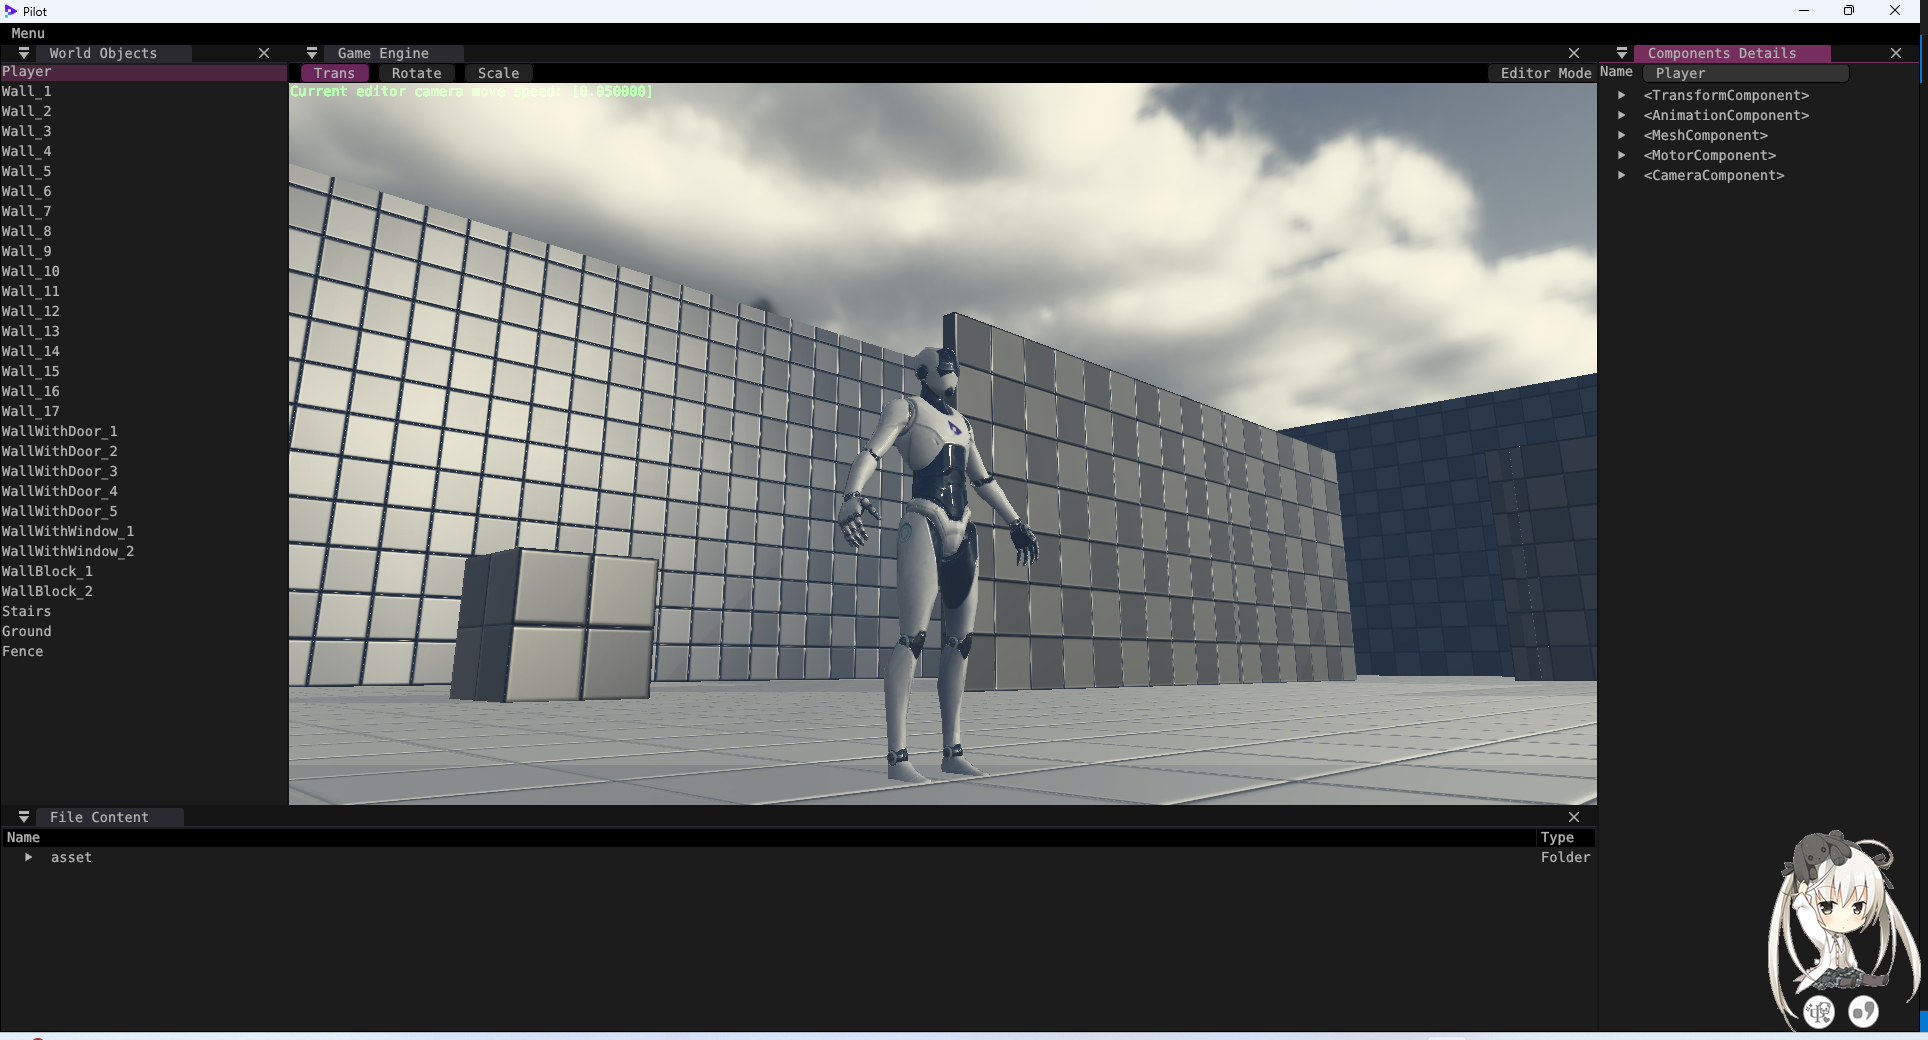
\includegraphics[width=\textwidth]{screen_shot_color_grading_map_color_grading_lut_01.png}
    	\end{subfigure}
    	\begin{subfigure}{1.0\textwidth}
    		
\includegraphics[width=\textwidth]{color_grading_lut_01.png}
    	\end{subfigure}  	
    	\caption{颜色分级效果截图color\_grading\_lut\_01.png}
    \end{figure}
     \begin{figure}[!htb]
    	\centering
    	\begin{subfigure}{1.0\textwidth}
    		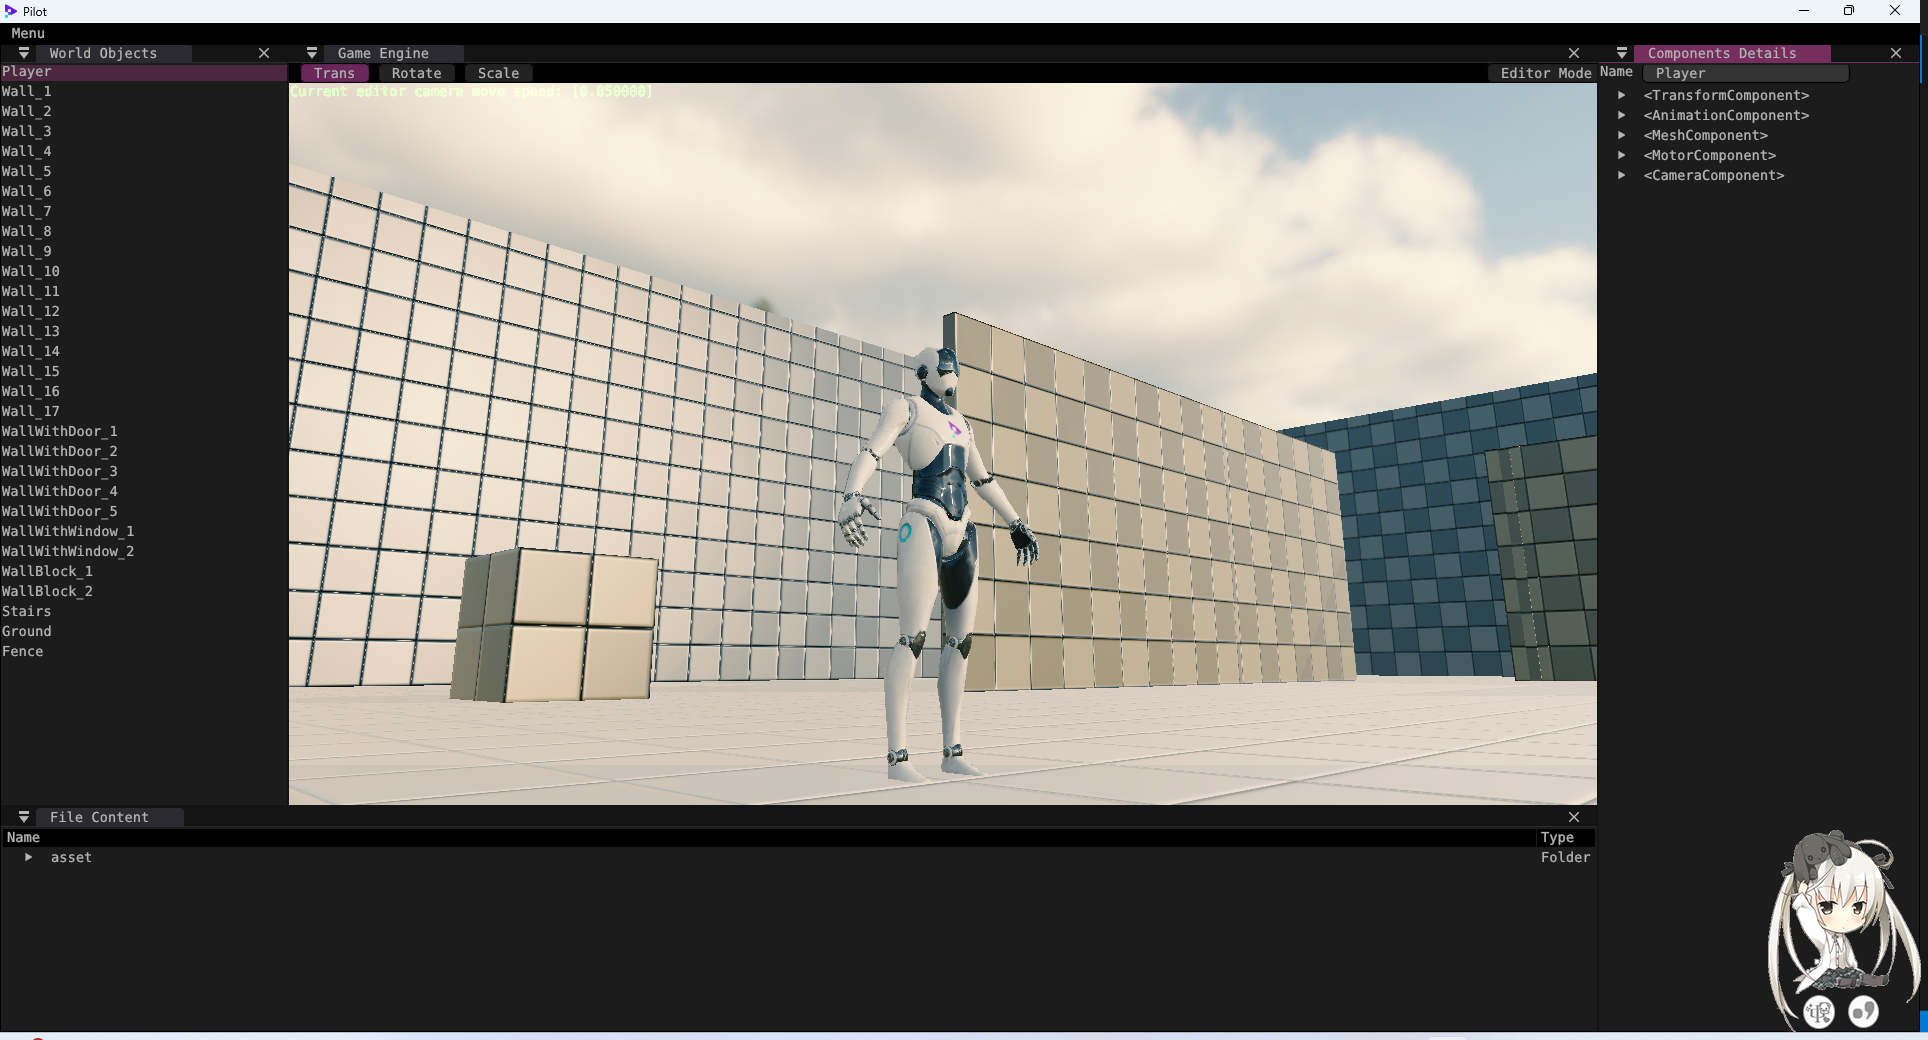
\includegraphics[width=\textwidth]{screen_shot_color_grading_map_color_grading_lut_02.png}
    	\end{subfigure}
    	\begin{subfigure}{1.0\textwidth}
    		
\includegraphics[width=\textwidth]{color_grading_lut_02.png}
    	\end{subfigure}  	
    	\caption{颜色分级效果截图color\_grading\_lut\_02.png}
    \end{figure}  
     \begin{figure}[!htb]
    	\centering
    	\begin{subfigure}{1.0\textwidth}
    		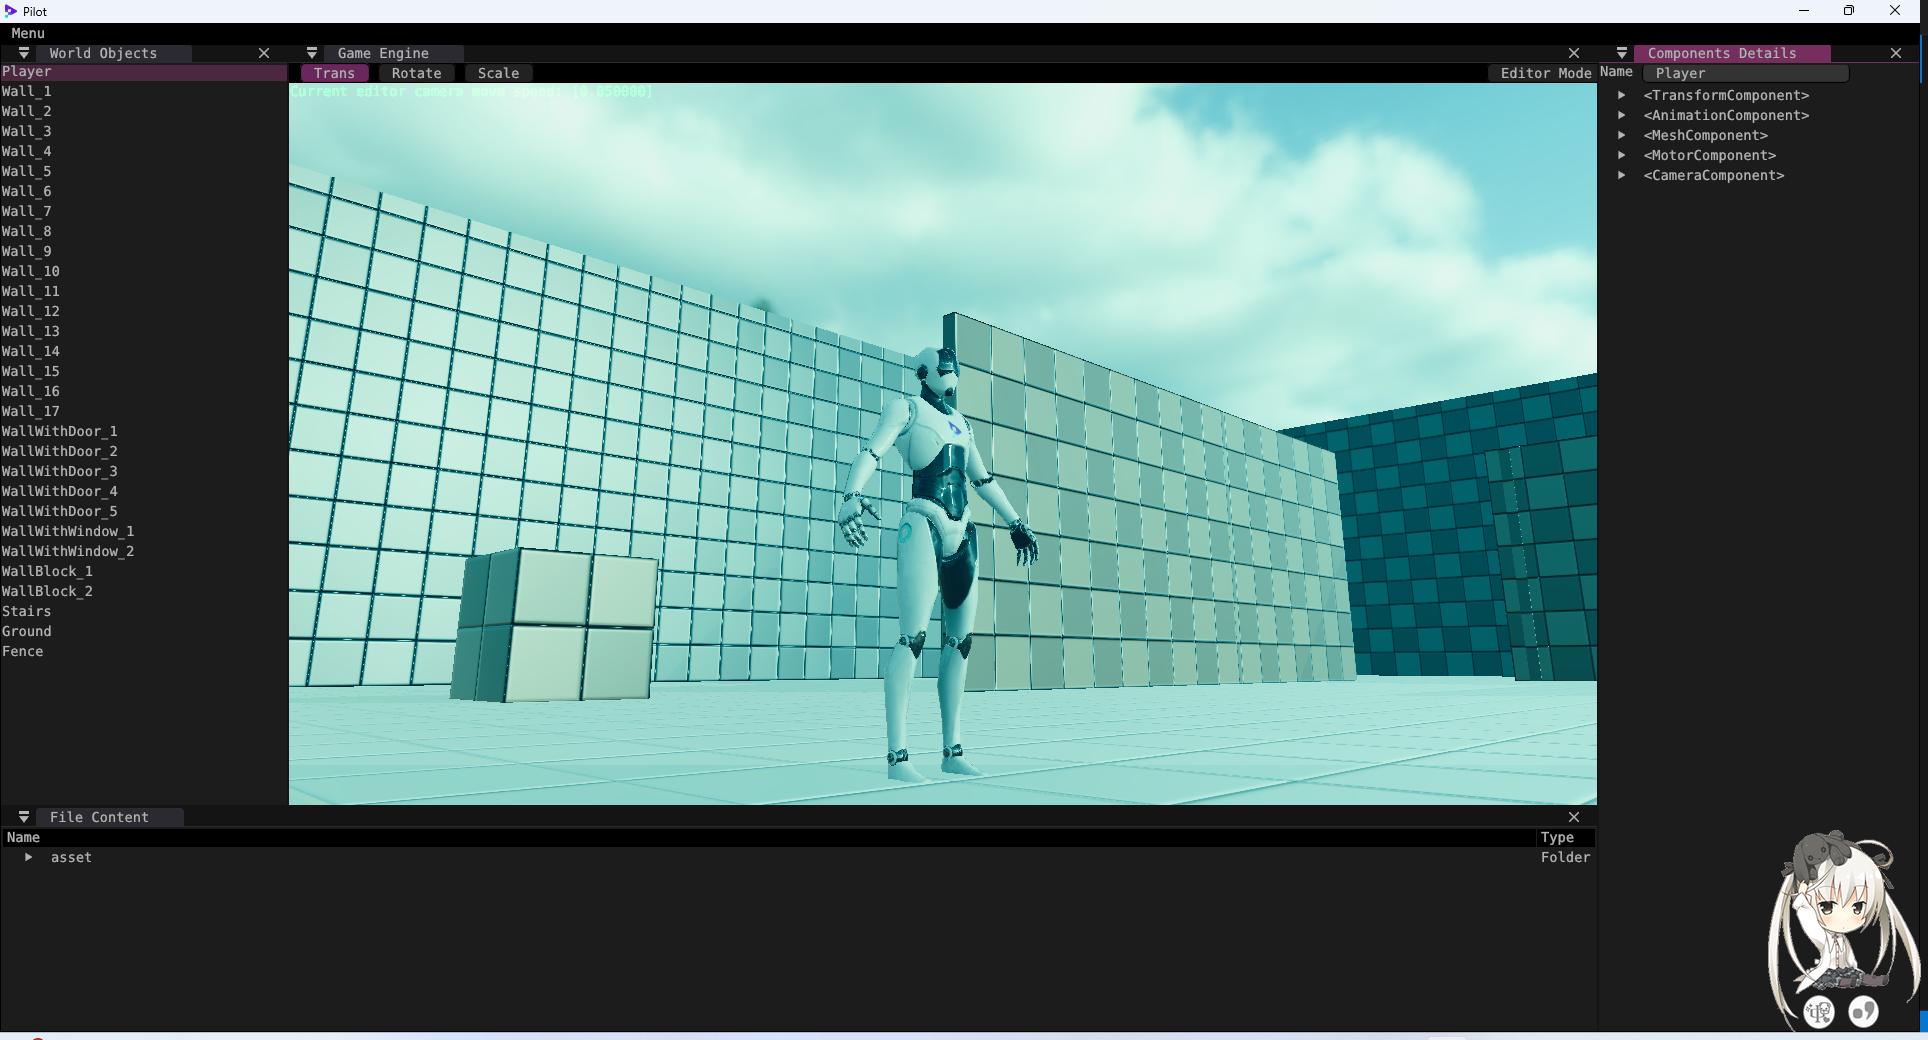
\includegraphics[width=\textwidth]{screen_shot_color_grading_map_color_grading_lut_03.png}
    	\end{subfigure}
    	\begin{subfigure}{1.0\textwidth}
    		
\includegraphics[width=\textwidth]{color_grading_lut_03.png}
    	\end{subfigure}  	
    	\caption{颜色分级效果截图color\_grading\_lut\_03.png}
    \end{figure}    
    \begin{figure}[!htb]
    	\centering
    	\begin{subfigure}{1.0\textwidth}
    		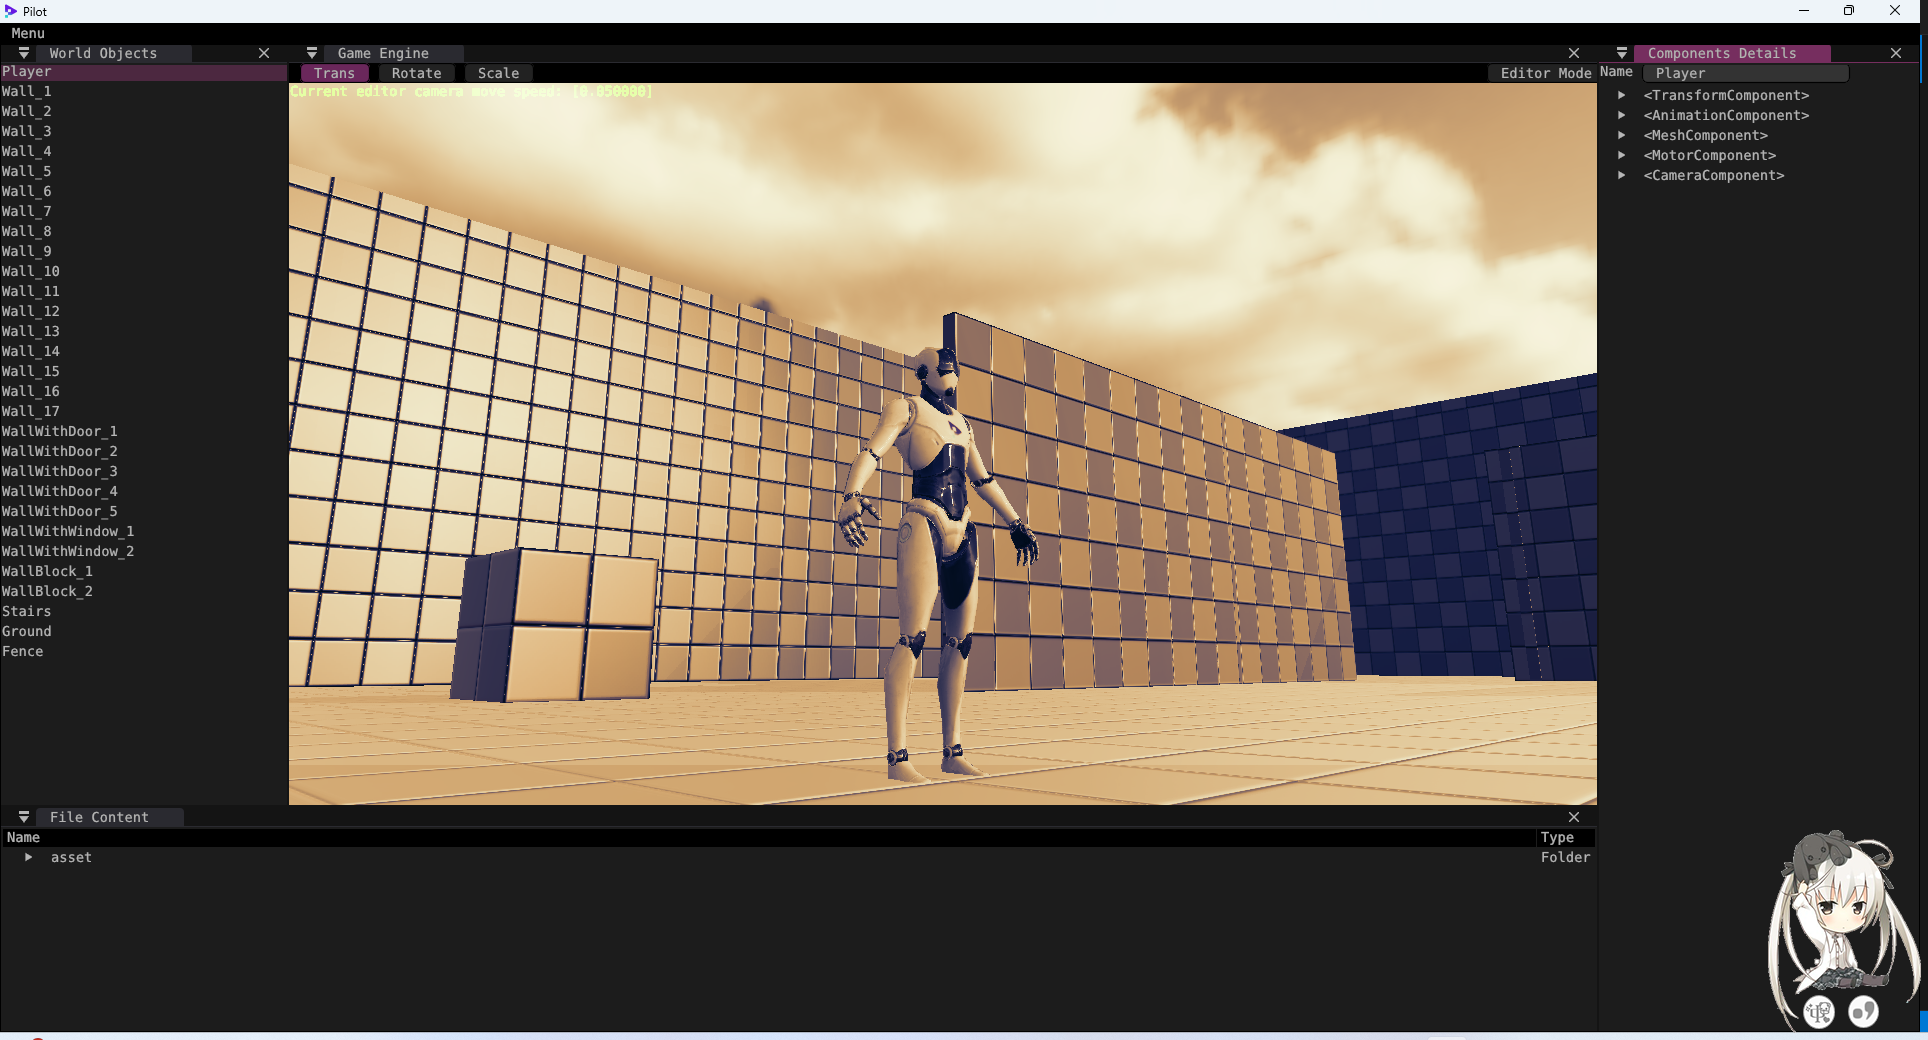
\includegraphics[width=\textwidth]{screen_shot_color_grading_map_color_grading_lut_04.png}
    	\end{subfigure}
    	\begin{subfigure}{1.0\textwidth}
    		
\includegraphics[width=\textwidth]{color_grading_lut_04.png}
    	\end{subfigure}  	
    	\caption{颜色分级效果截图color\_grading\_lut\_04.png}
    \end{figure}  
     \begin{figure}[htbp]
    	\centering
    	\begin{subfigure}{1.0\textwidth}
    		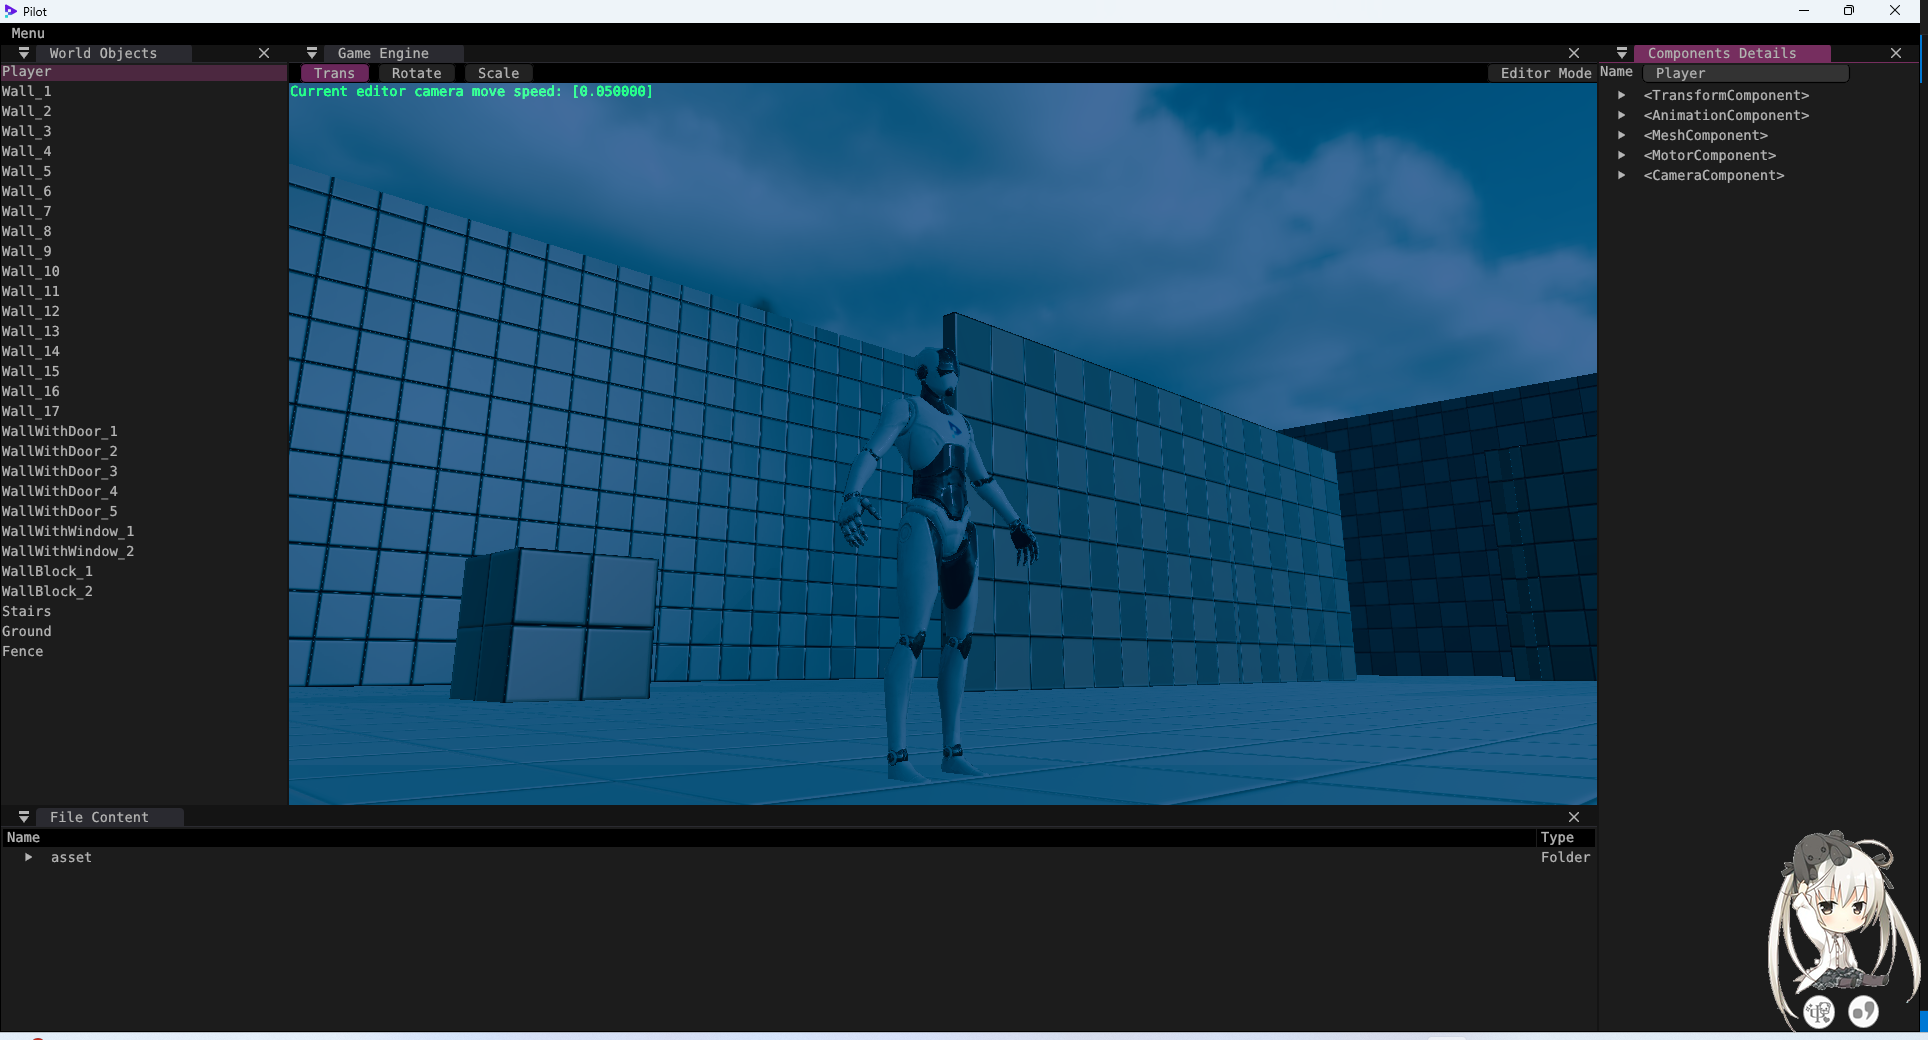
\includegraphics[width=\textwidth]{screen_shot_color_grading_map_color_grading_lut_05.png}
    	\end{subfigure}
    	\begin{subfigure}{1.0\textwidth}
    		
\includegraphics[width=\textwidth]{color_grading_lut_05.png}
    	\end{subfigure}
    	\caption{颜色分级效果截图color\_grading\_lut\_05.png}
    \end{figure}    
    \begin{figure}[!htb]
    	\centering
    	\begin{subfigure}{1.0\textwidth}
    		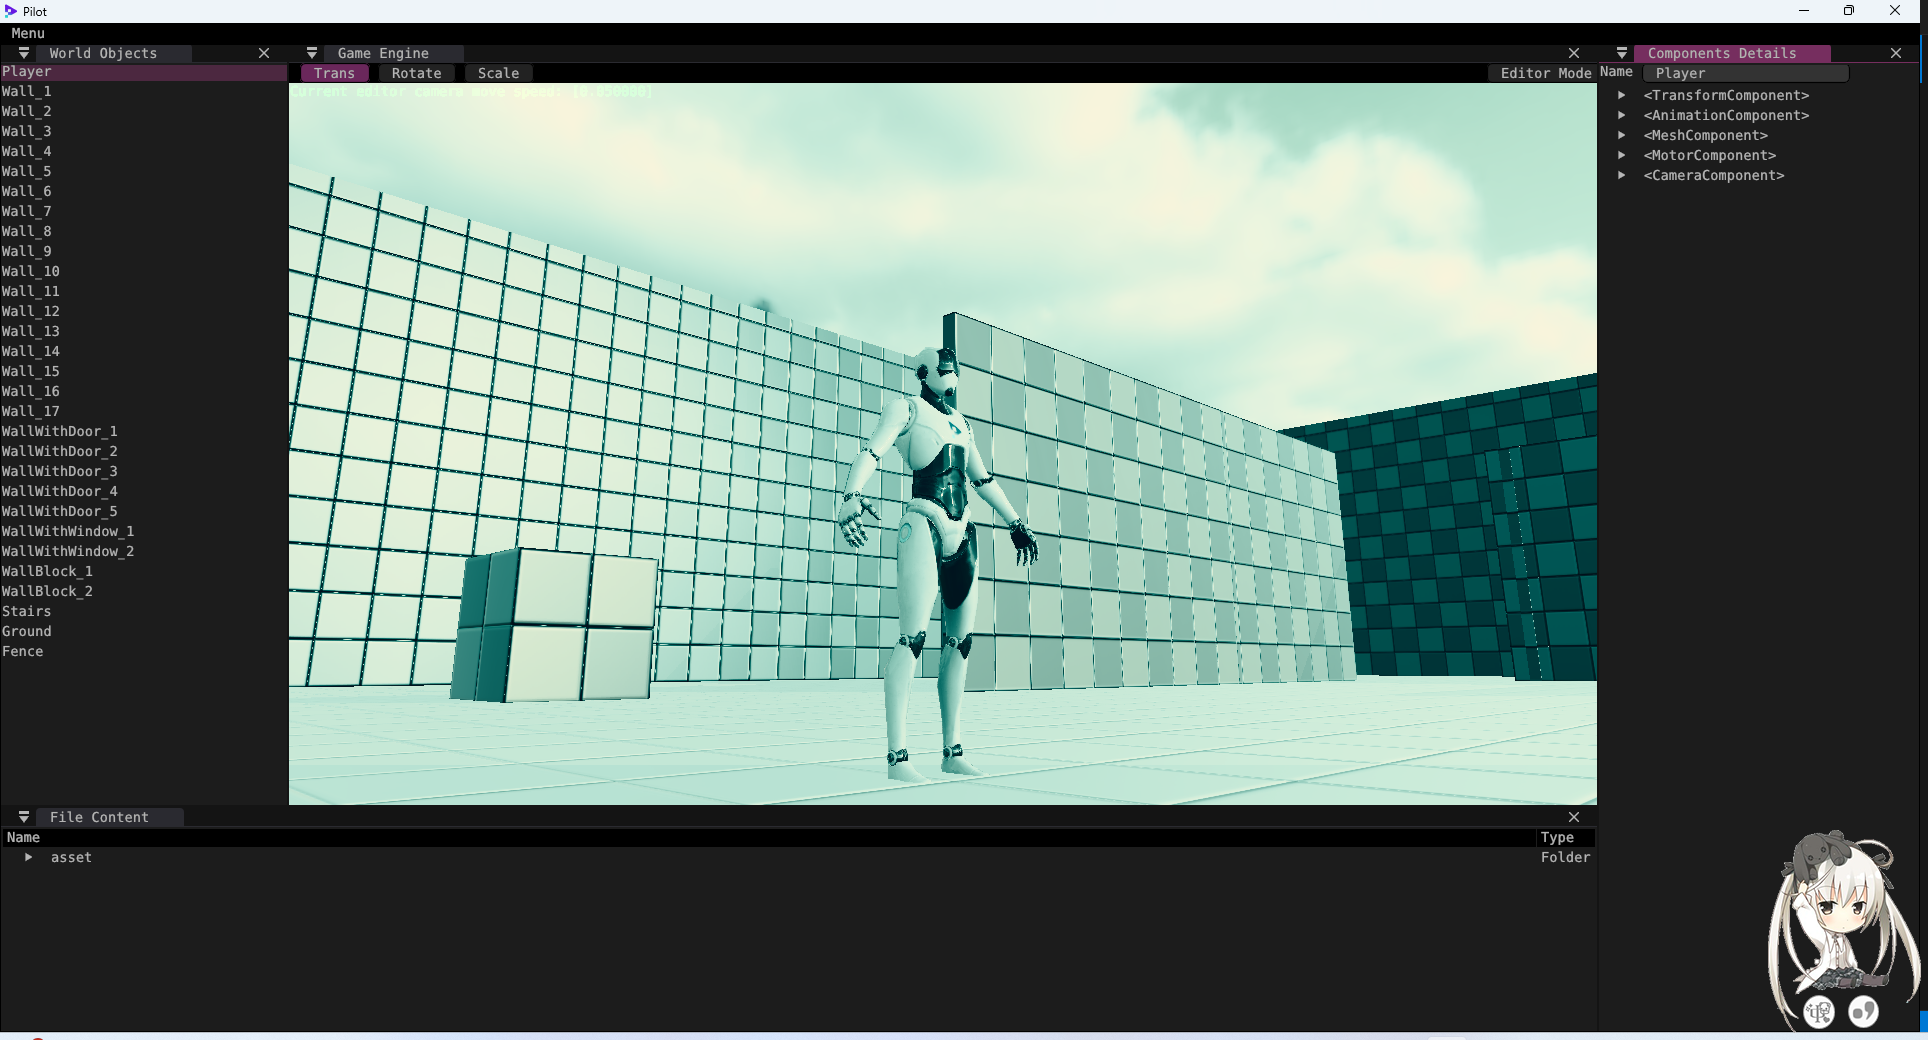
\includegraphics[width=\textwidth]{screen_shot_color_grading_map_color_grading_lut_06.png}
    	\end{subfigure}
    	\begin{subfigure}{1.0\textwidth}
    		
\includegraphics[width=\textwidth]{color_grading_lut_06.png}
    	\end{subfigure}  	
    	\caption{颜色分级效果截图color\_grading\_lut\_06.png}
    \end{figure}  
     
    \section{提高:后期处理}
     
     
\end{document}